\chapter{Progettazione}

\section{Interrogazioni}
\begin{table}[h]
\begin{tabular}{cll}
	\rowcolor[HTML]{333333} 
	{\color[HTML]{FFFFFF} \#} & {\color[HTML]{FFFFFF} Query}                                                                                       & {\color[HTML]{FFFFFF} Obiettivo}                                                                                                                                                                                                                   \\
	1                         & \begin{tabular}[c]{@{}l@{}}Impatto ambientale medio in corse\\ da 5 km (CO2 e NOx, massa)\end{tabular}             & \begin{tabular}[c]{@{}l@{}}Pensata per analizzare varianti della\\ stessa interrogazione su diversi livelli\\ di granularità\end{tabular}                                                                                                          \\
	\rowcolor[HTML]{C0C0C0} 
	2                         & \begin{tabular}[c]{@{}l@{}}Consumo medio per intervalli di\\ velocità prefissati, su tutto il dataset\end{tabular} & \begin{tabular}[c]{@{}l@{}}Utile all'implementazione e l'analisi\\ di viste materializzate che\\ raggruppano i dati secondo delle \\ fasce di velocità. Le fasce scelte, \\ espresse in km/h, sono le seguenti:\\ 0-50, 50-90, 90-130\end{tabular} \\
	3                         & \begin{tabular}[c]{@{}l@{}}Efficienza dell'auto per intervalli\\ di RPM (rotazioni per minuto)\end{tabular}        & \begin{tabular}[c]{@{}l@{}}Altra interessante interrogazione\\ creata allo scopo di sfruttare le\\ viste materializzate. Il dataset \\ fornisce tutti i parametri \\ necessari al calcolo dell'efficienza, \\ o rendimento istantaneo\end{tabular} \\
	\rowcolor[HTML]{C0C0C0} 
	4                         & \begin{tabular}[c]{@{}l@{}}Per ogni test, media di NOx,\\ CO2, Potenza e Velocità\end{tabular}                     & \begin{tabular}[c]{@{}l@{}}Quest'interrogazione serve a\\ valutare le prestazioni ottenute\\ dall'esecuzione su di un \\ partizionamento verticale con le\\ colonne sparse tra più tabelle\end{tabular}                                            \\
	5                         & \begin{tabular}[c]{@{}l@{}}Media e deviazione standard\\ delle temperature\end{tabular}                            & \begin{tabular}[c]{@{}l@{}}Quest'interrogazione serve a \\ valutare le prestazioni ottenute\\ dall'esecuzione con le colonne \\ concentrate su di un unica\\ tabella restituita da un\\ partizionamento verticale\end{tabular}                    
\end{tabular}
\end{table}

\section{Diagrammi}
\begin{figure}
	\centering
	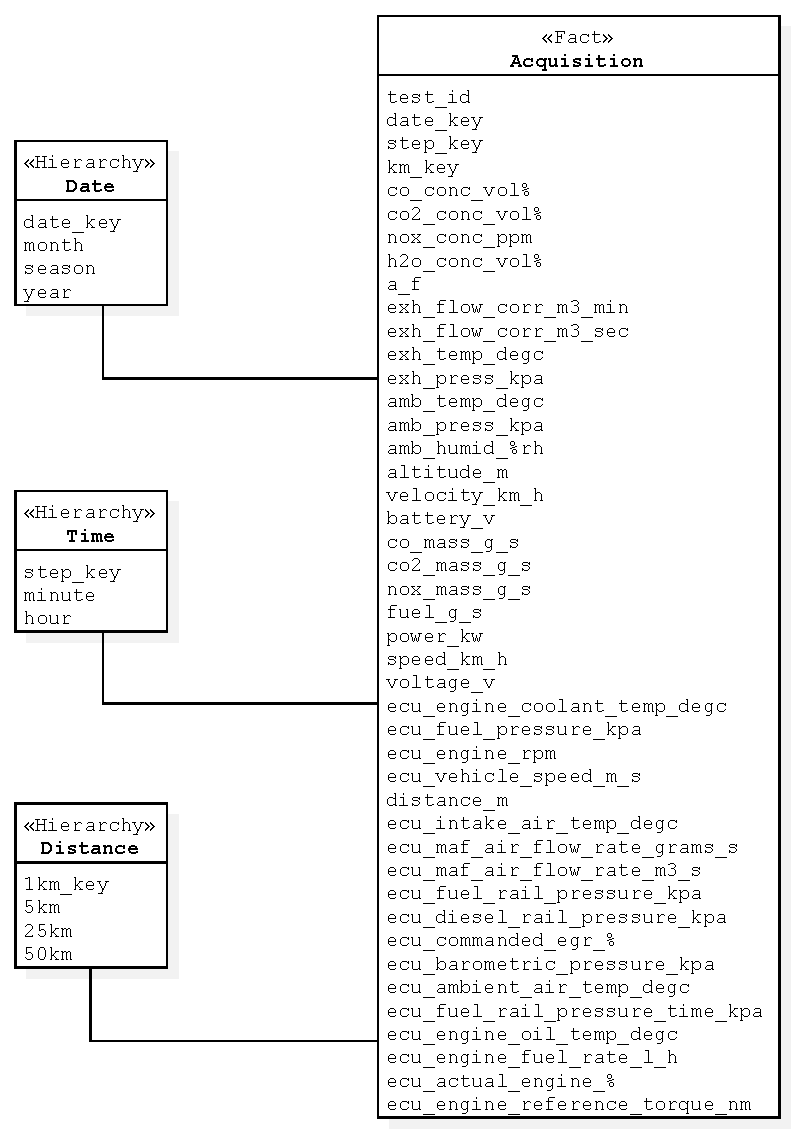
\includegraphics[width=1.\linewidth]{figures/class_fact_scheme}
	\caption{}
	\label{fig:ofm}
\end{figure}
